\subsection{Formal Modeling}
This section is dedicated to the Formal Modeling phase description. The Section is divided in Schema and Data level in order to report the details regarding both the ontology generated and the datasets version in the current phase.

\subsubsection{Schema level}
The schema level section in the current phase, reports the detailed description of the ontology generation.

\paragraph{Ontology definition}\mbox{}\\
The first step in the process of developing an ontology schema is to search for other reference ontologies. In this project, there are few reference examples, but we have the a priori knowledge that the data crawled from different websites are cell names and their related attributes. It is common knowledge that, within a given range, cell names can help people to identify different cells, so cell names and cell entities correspond to each other. In addition, the cell names are given by the cell entities themselves, and the websites are only responsible for collecting and organizing the relevant information without subjective processing, so the cell name attribute fields of the heterogeneous databases completely overlap and there is no ambiguity, which brings convenience to the data level fusion.


A simplest approach is adopted in this project, i.e., multiple databases are stitched together as the database after fusion based on the cell name restriction. The pseudo python code of the algorithm is shown 
as follows.


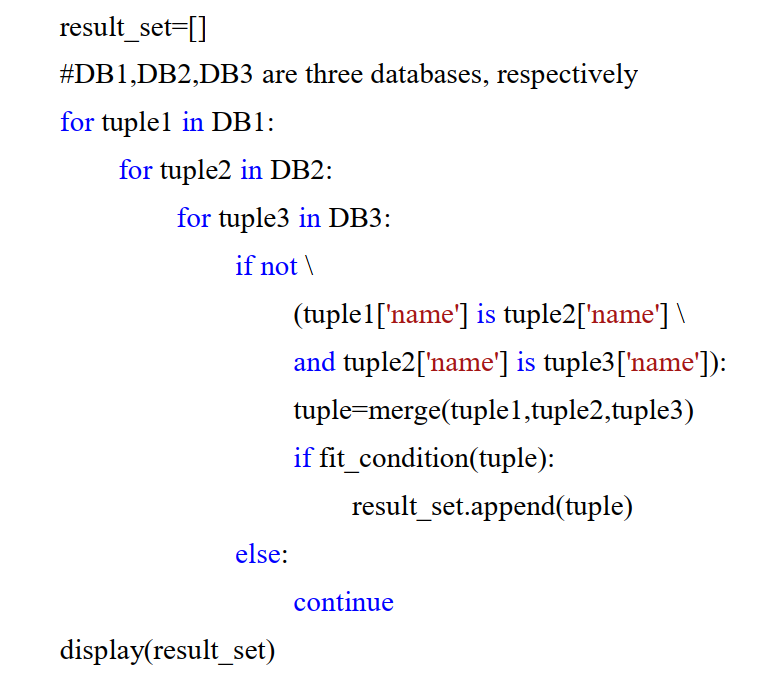
\includegraphics[width=8cm]{student codebook/sections/figure.png}
    \caption{python pseudo-code of our algorithm}



